\renewcommand{\thefigure}{A\arabic{figure}}
\setcounter{figure}{0}
\renewcommand{\thetable}{A.\arabic{table}}
\setcounter{table}{0}
\renewcommand{\thesection}{A.\arabic{section}}
\setcounter{section}{0}

\section*{Appendix}

\subsection*{PTS Civil War Robustness Check}

\begin{figure}
    \centering
    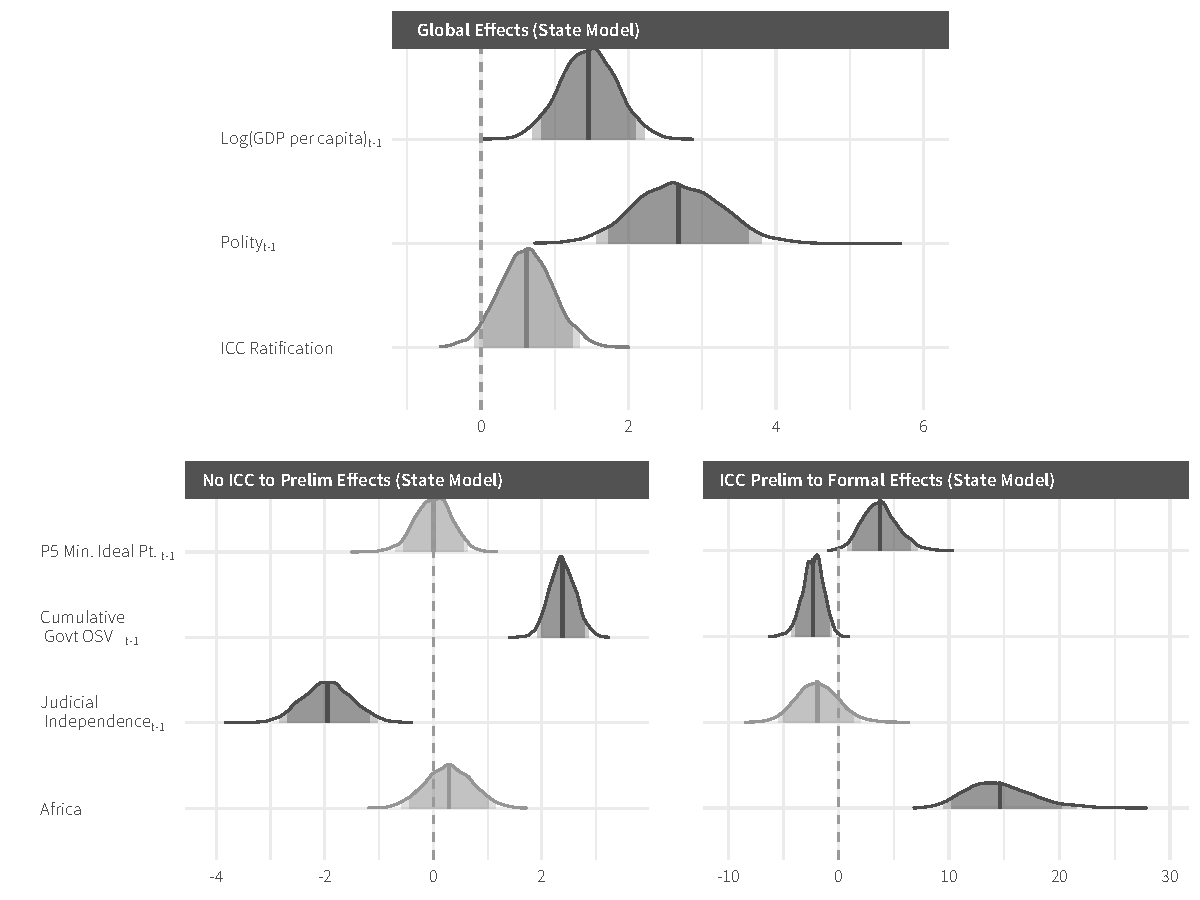
\includegraphics[width=1\textwidth]{stateCoefSumm_ptsCivilWarOnly.pdf}
    \caption{Parameter estimates from State-Focused ICC Transition model visualized through posterior distributions with median values designated by vertical line, lightly shaded portion indicating the 95\% credible interval, and darker shaded portion the 90\% credible interval.}
    \label{fig:stateModel}
\end{figure}

\begin{figure}
    \centering
    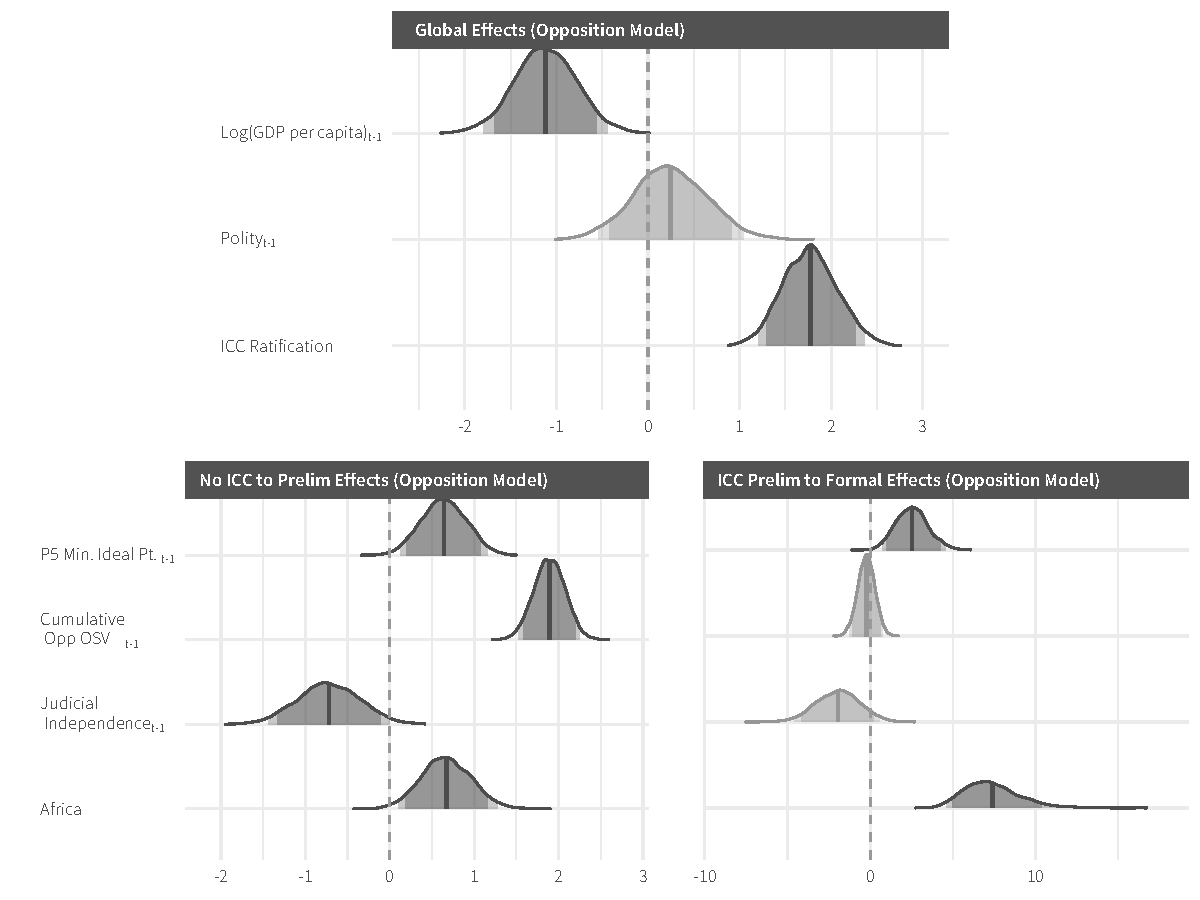
\includegraphics[width=1\textwidth]{rebelCoefSumm_ptsCivilWarOnly.pdf}
    \caption{Parameter estimates from Opposition-Focused ICC Transition model visualized through posterior distributions with median values designated by vertical line, lightly shaded portion indicating the 95\% credible interval, and darker shaded portion the 90\% credible interval.}
    \label{fig:rebelModel}
\end{figure}

\subsection*{Comparison with ordinal logit}

\begin{figure}
    \centering
    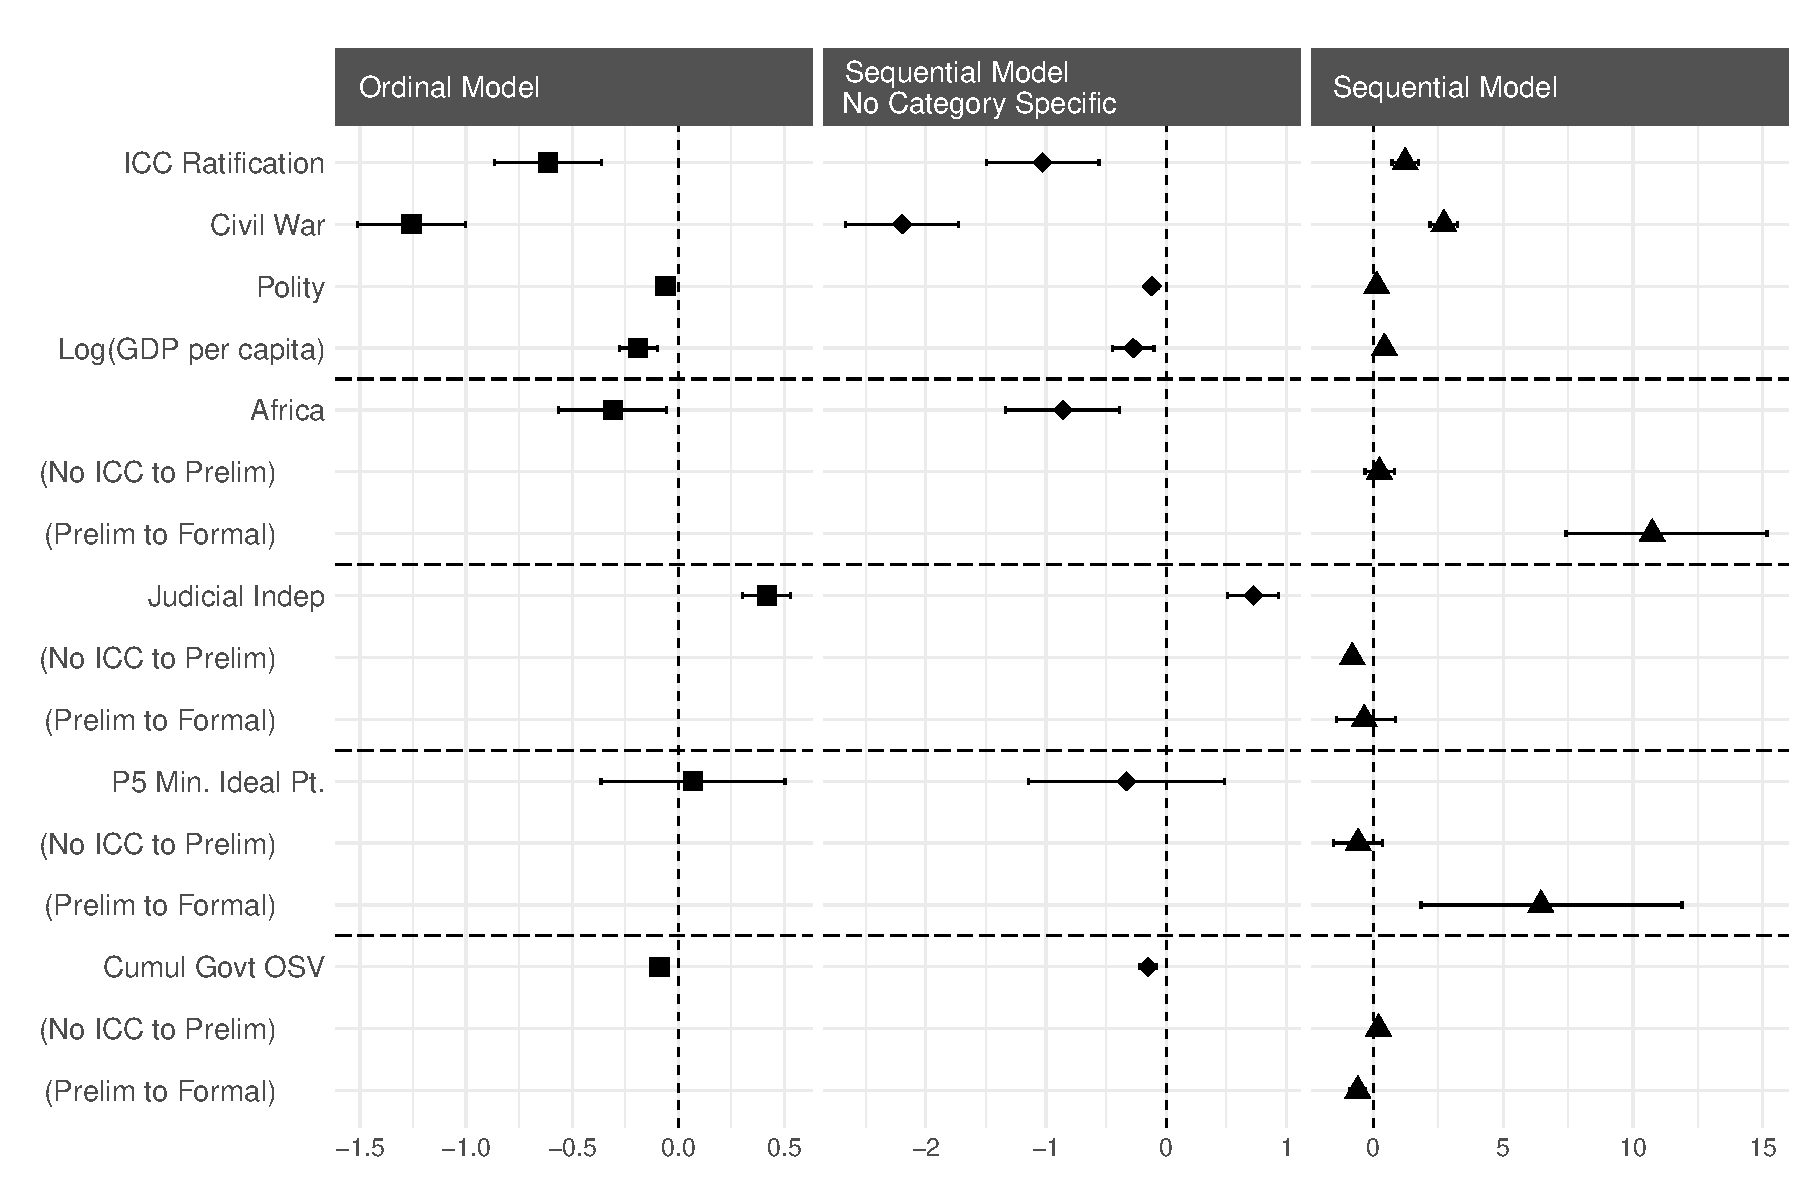
\includegraphics[width=1\textwidth]{modCompare_state.pdf}
    \caption{State model.}
    \label{fig:stateCoefCompare}
\end{figure}

\begin{figure}
    \centering
    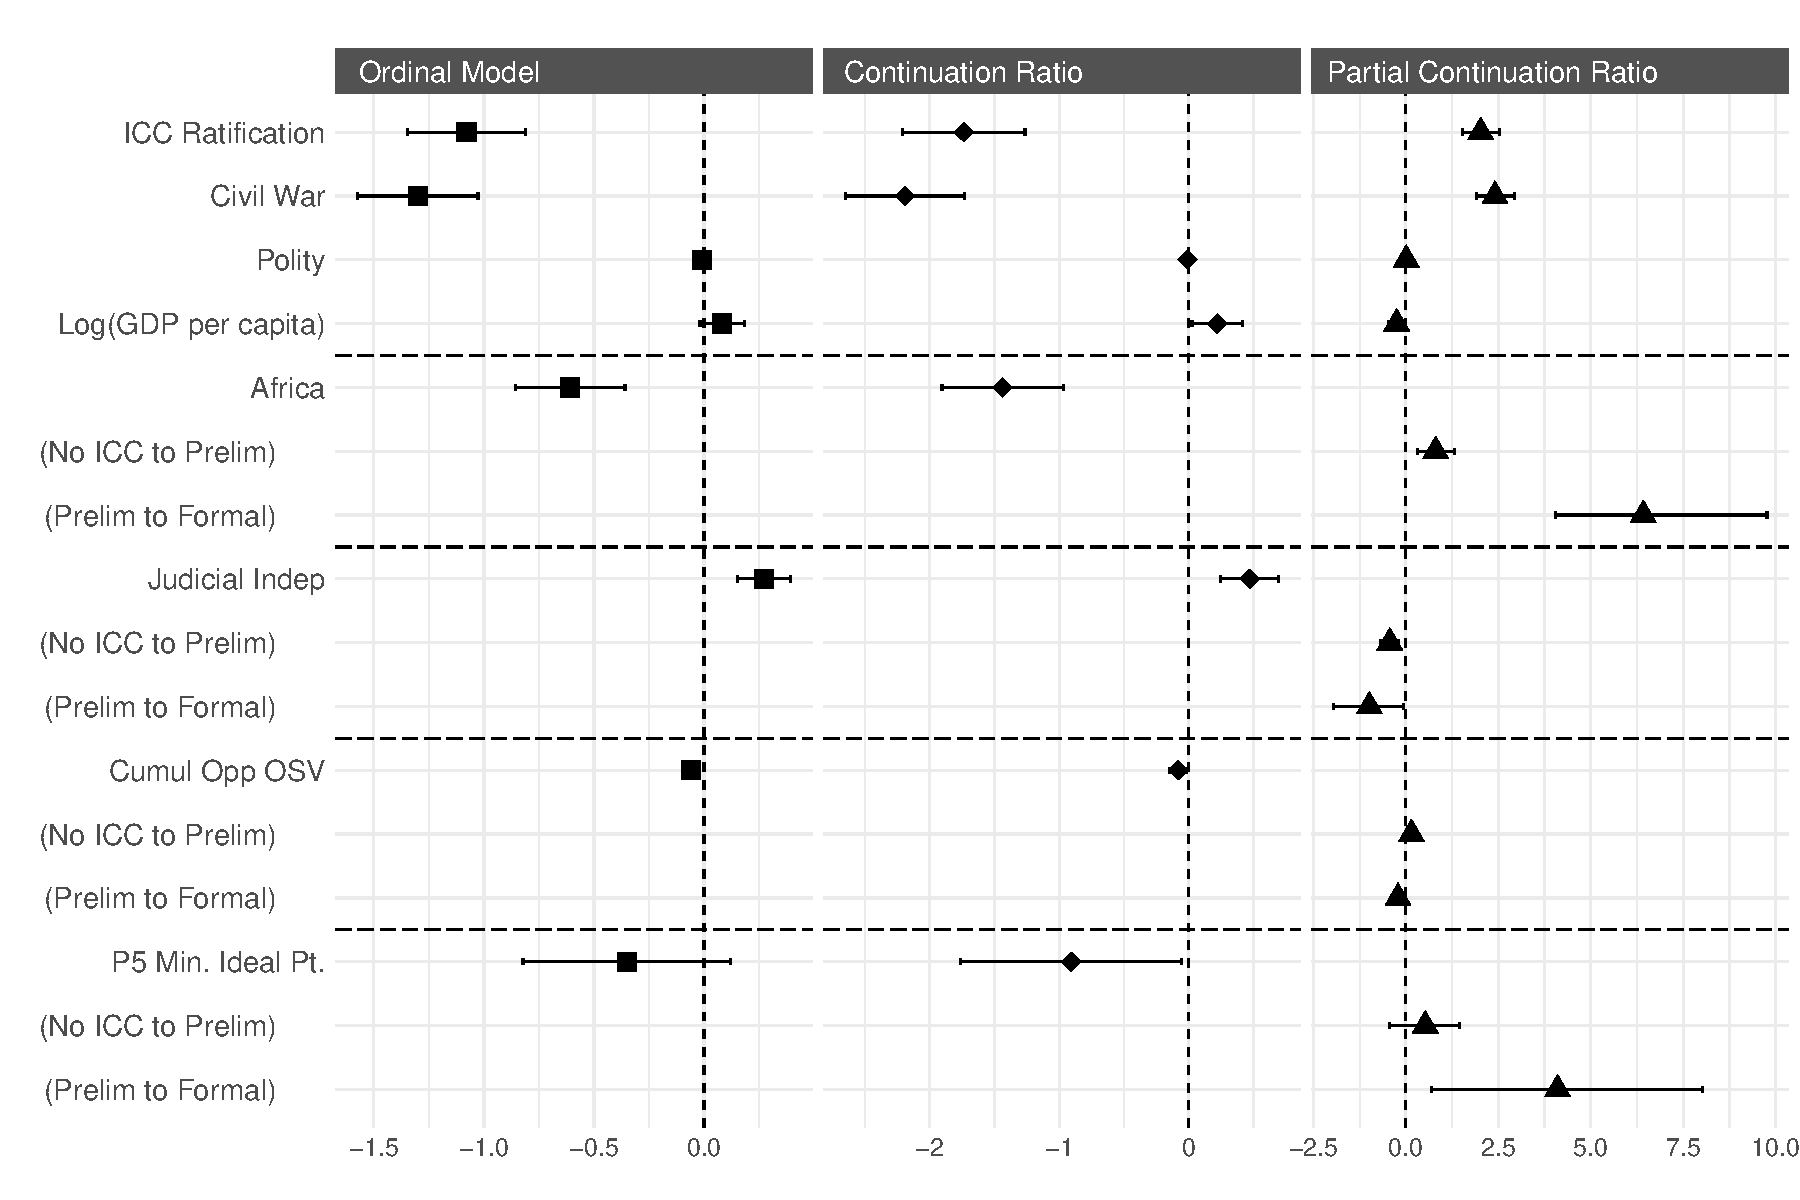
\includegraphics[width=1\textwidth]{modCompare_opp.pdf}
    \caption{Opposition model.}
    \label{fig:oppCoefCompare}
\end{figure}

For ordinal variables such as the CIRI components the choice of a fit statistic is not as obvious. We use Somer's $D$, a rank correlation coefficient  \citep{Somers1962}, as our discrepancy statistic for the ordinal logit models.
Somer's $D$ is closely related to Goodman and Kruskal's $\gamma$ and Kendall's $\tau$, differing only in the denominator.\footnote{Somer's $D$ is similar to the commonly used $\tau_b$, which is equal to $\frac{P - Q}{(P+Q+X_0)(P+Q+Y_0)}$, where $Y_0$ is the number of ties in $Y$, and $\gamma$, which is equal to $\frac{P - Q}{P + Q}$.} Somer's $D$ makes a distinction between the independent and dependent variable in a bivariate distribution, correcting for ties within the independent variable. With $Y$ being treated as the independent variable it is denoted $D_{xy}$.

Specifically:
$$D_{xy} = \frac{P - Q}{P + Q + X_0}$$

\noindent where $P$ is the number of concordant pairs, $Q$ is the number discordant pairs, and $X_0$ is the number of ties in $X$. This is simply a measure of association for ordinal variables, so our approach is essentially to calculate the correlation between predicted and observed values. Like all correlation coefficients, the $D$ statistic lies in the interval $[-1, 1]$, with values closer to $1$ indicating more rank agreement and values closer to $1$ indicated less rank agreement, so values closer to 0 indicate more prediction error. In the results section below we discuss how we use these performance measures to judge whether covariates add substantially to a model's predictive ability.

\begin{figure}
    \centering
    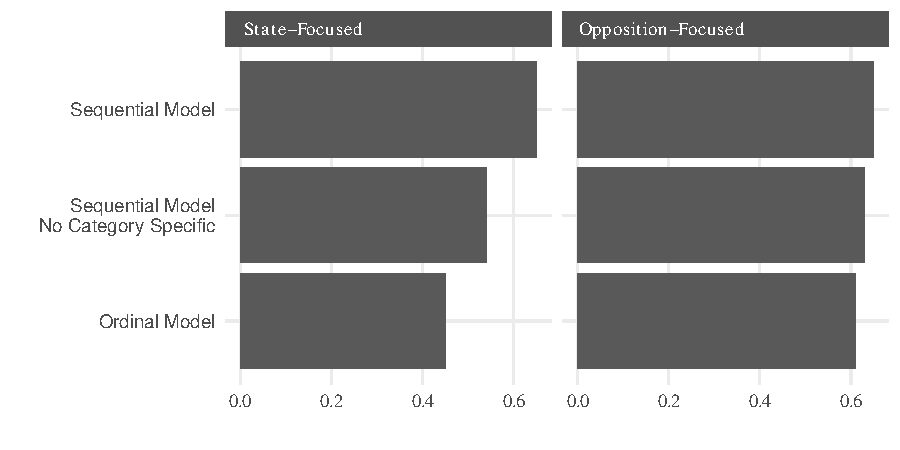
\includegraphics[width=1\textwidth]{somerViz.pdf}
    \caption{Performance comparison.}
    \label{fig:somersD}
\end{figure}

\subsection*{MCMC sampler}


\subsection*{Stan Code}
